\chapter{Method of Approach} 
\label{ch:method}



\section{Brief Overview}
\hspace{20pt}In this project, the objective is to create an eight-year panel-data analysis for 12 countries. These countries come under the category of developed, emerging, and low-income economies. To have a global perspective, these countries are chosen in a way that resembles regions worldwide, including East Asia & Pacific, Europe & Central Asia, Latin America, Middle East, and Africa, North America, South Asia, and Sub-Saharan Africa.

\section{Country Classification by Income Level and Years}
\hspace{20pt} The World Bank classifies the world’s economies into four income groups: high-income, upper-middle-income, lower-middle-income, and low income. This classification is based on the Gross National Income (GNI) per capita, which is currently measured in US\$ []. The GNI is a measure of the total income earned by the people and businesses, whether they are located within the nation or abroad [def. Investopedia]. The GNI per capita for high-income countries is greater than \$12,375, whereas the GNI per capita for upper-middle-income countries is between \$3,996 and \$12,375. For lower-middle-income-countries, the GNI ranges from \$1,026 to \$3,995, and for low-income countries, it is lower than \$1,026. This thesis focuses on the first three categories: high-income, upper-middle-income, and lower-middle-income.

High-Income economies are advanced with better infrastructure, mature capital markets, and most importantly, high household incomes. Multinational corporations are attracted to such economies, and they tend to invest heavily, leading to accelerated economic growth and job opportunities. Next, upper-middle-income are in rapid growth, but in comparison to high-income, they have lower capital markets and lower household incomes. The progress of an upper-middle economy allows it to engage more with the global market, leading to increased trade and foreign direct investment (FDI). In short, upper-middle-income (also called emerging economies) are transitioning towards becoming a high-income economy. The next category that has been defined in this project is lower-middle-income economies. These countries struggle to provide basic necessities such as food and water, have limited access to education, and low returns to work. Based upon this classification, the final list of countries created for this study is included in the table below.

\begin{table}[h!]
    \centering
    \begin{tabular}{|c|c|}
    \hline
    \textbf{Country } & \textbf{Category} \\ [0.5ex] 
 \hline\hline
 United States & High-Income \\ 
 \hline
 Germany & High-Income \\
 \hline
 Australia & High-Income \\
 \hline
 Japan & High-Income \\
 \hline
 Israel & High-Income \\
  \hline
 China & Upper-Middle Income \\
 \hline
 India & Upper-Middle Income \\
 \hline
 Russia & Upper-Middle Income \\
 \hline
 South Africa & Upper-Middle Income \\
  \hline
 Mexico & Upper-Middle Income \\
 \hline
 Nepal & Lower-Middle Income \\
 \hline
 Nigeria & Lower-Middle Income \\
 \hline
    \end{tabular}
    \caption{Categorization of Economies Based on the Level of Income}
    \label{tab:my_label}
\end{table}

For the panel-data analysis, the data has been extracted from 2012 to 2019. The Great Recession of the year 2007 cast a long shadow over the economic expansion that followed. The world’s financial markets took the biggest hit, along with the banking and real estate industries. The recession led to an increase in home mortgage foreclosures, and millions of people were in a situation where they were losing their life savings, jobs, and homes. In 2012, the World Economic situation and Prospects mentioned that after much turmoil during 2011 global capital markets gained some stability in early 2012. During the first quarter of 2012, some high-income economies such as United States, Japan, and Germany were predicted to have some calming financial markets and were expected to recover moderately. Furthermore, most middle-income economies expected less volatility in private capital inflows, more moderated swings in exchange rates and modest stock market gains. The state of the global economy was fragile, and despite the circumstances, the world progressed slowly and steadily. Each economy in the world has transitioned differently following the years of the economic crisis. In addition to the trends of the transition, the analysis over those years will further spark light on how an economic situation of a country allows it to rise above the circumstances and how the resources available to help them get on on the right track.

\section{Dependent and Independent Variables}
\hspace{20pt} It is crucial to analyze the gap between countries to understand why some countries are rich and why others are poor. In doing so, multiple factors or variables will be used to search for the cause and effect relationship to identify why things are a certain way and use those insights to get reliable predictions. We have classified our variables as dependent and independent variables. The dependent variable is the variable that is being tested and measured for this thesis is income inequality, and its value will be affected by independent variables. On the other hand, the independent variable is the variable that will be manipulated by us and is assumed to have a direct effect on income inequality. In this study, those effects are led by Skill-Biased Technological Change and Globalization.

\subsection{Dependent Variable}

\hspace{20pt} Studies show that income inequality is a condition that prevails along with economic growth. Earlier, we discussed the inverted  U-shaped Kuznets curve that showed that income inequality is the lowest at the initial level of low economic growth. As the nation’s economic growth progresses, income inequality increases until a threshold level and decreases with increased economic growth. Our study is based on the idea that economic growth has an impact on income inequality. GDP is considered to be the single best indicator of economic growth. In a study conducted to understand the relationship between annual GDP growth and income inequality in developed and developing economies, a linear relationship was found \cite{luan2017relationship}. The study further serves as an understanding of what countries could expect to happen based on their GDP. 

A country's GDP accounts for the total value of goods and services produced within a country's borders during a specific period. Breaking down this output and dividing it by a country's population leads us to GDP per capita. The metric shows how much economic production value can be accounted to the citizens of the country. Furthermore, it helps with a better analysis of the average living standards and well-being when comparing countries. A citizen is supposed to be doing well financially when they have acceptable living standards, which can be accounted for through their income. Hence, this measure of economic activity will be acquired from the World Bank’s website


\subsection{Independent Variable}

To analyze the impact of Skill-Biased Technological Change and Globalization on our dependent variable, GDP per Capita, the following list of factors that will be accounted as our independent variables.

\begin{enumerate}
\item \underline{\textbf{Expenditure on Research and Development (R\&D)}}: 

Research and Development (R\&D) is a significant factor contributing towards technological advancement across nations. It is a process that has the incentive to create new or improved technology to provide a competitive advantage at the business, industry, or national level, hence playing a crucial role in GDP growth. A study conducted on some selected OECD countries showed that R\&D expenditures positively and significantly impact economic growth \cite{surani2017economic}. R\&D expenses support a lot of industrial, technological, health care, and pharmaceutical sectors. Many economists agree that innovation can lead to higher productivity for workers, leading to increased wages, improved quality of life, and greater output for the economy. These industries are also the ones to be most impacted by skill-biased technological changes. As a result of R\&D, when new tools and machinery are integrated within the manufacture of products and services, the demand for high-skilled laborers who can adjust to the change increases. To gain a competitive advantage and economies of scale, the countries and firms have an incentive to provide innovative and efficient products or services that will gain recognition at the national and international markets. Hence, they tend to invest a lot within R\&D. The data for R\&D (as a percent of GDP) is accessible from the World Bank's database.

\item \underline{\textbf{Availability of Scientists and Engineers:}}

Development within nations has been linked with advancements in science and technology. Nations that have a large number of citizens involved in generating knowledge and creating technology do not have to rely on other countries to develop new tools. This variable is used as an indicator to calculate the availability of highly educated human resources available in a given country. People in such positions are experts in applying scientific and technical knowledge and play a vital role in the economy’s sustained growth and stability. They are collectively regarded as a nation’s highly qualified workforce and contribute towards understanding and solving some of the complex challenges faced by a business, industry, or country, which often involves developing new technologies. A Wall Street Journal article noted that the quality of scientist and engineers and their proximity to research centers is crucial to multinational corporations \cite{onyeiwu2008does}. The variable will play an essential role in identifying how technological leadership affects a nation’s economic strength. We will access this data from UNESCO’s (United Nations Educational, Scientific and Cultural Organization) database. This variable’s value will range from one to seven, one being scarce and seven being widely available

\item \underline{\textbf{Expenditure in Education:}}
Education is an essential identifier of economic growth and development. Educated citizens have access to a wide range of opportunities compared to those who are not, and it becomes easier for them to adapt to the changing environment. Broad availability of quality education is a foundation for future training as people transition to new jobs \cite{international2010skilled}. One of the best predictors of an individual’s income is educational attainment; hence a nation’s strategic policies towards investment in education could equip the skills required for the jobs of today and tomorrow \cite{mayer2010relationship}. Especially in low-income nations, lack of education can lead to increased poverty and slow economic development. With access to better educational programs, citizens of a country can earn skills and apply them to their country’s development. According to a recent OECD report, providing every child with access to education and the skills needed to participate fully in society would boost GDP by an average of 28\% per year in lower-income countries and 16\% per year in high-income countries for the next 80 years \cite{writtenbyborgebrende}. The data for a country’s expenditure on education will be accessed from the World Bank’s database.

\item \underline{\textbf{High Technology Exports:}}

The strong emphasis on investments in research and development, largely in manufacturing and production sectors, has led to the creation of high technology products, leading to high technology exports, which significantly impact economic well-being. High-technology exports are products that have an R&D intensity and such exports include aerospace, computers, pharmaceuticals, scientific instruments, electrical machinery etcetera. Developing countries are the popular exporters of such products. A study by Connolly provides empirical evidence that high technology goods imports from developed countries not only positively affect domestic innovation, but also lead to increased GDP growth as higher quality capital goods are used in domestic production \cite{gani2009technological}. Implementation of these technologies makes the production process efficient on the one hand. On the other hand, the operation of such technologies takes away low-level jobs and instead favors more skilled jobs. We will acquire the data set for this variable from the World Bank's database.

\item \underline{\textbf{Number of Exports and Imports:}}
International trade, as an engine of economic growth, has gained a lot of interest. It allows a country to promote efficient allocation of resources, foster technological progress, gain competitive advantage, and achieve economies of scale. A country's imports and exports have a massive role in influencing the GDP per capita. A neoclassical growth modeling framework investigated the contribution of exports and imports to economic growth in a few European Union economies; the results suggested a positive relationship \cite{awokuse2007causality}. With more and more countries being open towards free trade, the consumers from all these countries can enjoy low-prices and various goods and services that encourage economies to involve more in import and export activities. However, some studies suggest based on the country’s trade, and economic structure, an increase in trade could result in income disparities \cite{rosenfeld2019international}. This variable will be used to analyze the economic progress and investigate how expensive or beneficial this shift can be for a nation’s workers. The data will be accessed from the World Bank's database.

\item \underline{\textbf{Foreign Direct Investment (FDI):}}

A foreign direct investment (FDI) happens when a business firm or individual in one country shows business interests in another country. Such interest is specifically essential for developing and emerging economies that do not have sufficient funding to expand their businesses. A case study on Pakistan was conducted to analyze the impact of FDI on GDP using a regression model, and a positive relationship was established \cite{iqbal2014impact}. FDI brings technological expertise within various industries that influence economic growth. In 2017, developing countries received \$671 billion, or 47\% of total global FDI. Investments rose 9\% in developing Asia, which received \$476 billion \cite{nachum2001united}. The recipient countries see growth in jobs and standard of living. Few consequences of FDIs significant to this thesis include trade deficits and disruption of domestic business practices. For instance, a state-level panel data analysis conducted in the US led to the conclusion that FDI can positively affect income inequality within some states \cite{chintrakarn2012fdi}. The relationship between FDI, GDP, and income inequality has been relatively ambiguous. The data for this variable will be accessed from the world bank’s database.

\item \underline{\textbf{Gross Capital Formation (GCF) (\% of GDP):}}

Gross Domestic Capital formation refers to the net investment in physical assets for a particular year for an economy. The asset includes factories, machinery, plants, equipment, and materials that can increase the physical capital stock of the nation. The increase in capital formation can provide a country’s population with necessary production tools, stimulate technological progress, and increase labor productivity, leading to an increased output level for the nation. It determines the national capacity to produce, which in turn affects economic growth. A research paper implemented the Ordinary Least Squares Technique (OLS) to investigate the impact of capital formation on Nigeria’s economic growth and showed a positive relationship \cite{ugochukwu2013impact}. It can be argued that deficiency of capital and acts as a barrier in the production of goods and services. The data for this variable will be accessed from the world bank’s database.

\item \underline{\textbf{Openness to Trade:}}

Prior to defining trade relationships with a country, it is important to look at what extent is the country “open” to defining its commercial relations with the rest of the world. The degree of openness is heavily impacted by the overall political, economic, and legal situation of a country. There are different degrees of openness based on the restrictions imposed by the country on free trade. A higher degree of openness can lead to new market opportunities for domestic firms, job opportunities for people, poverty reduction, and prominent economic growth. According to the World Bank, no country has thrived in modern times without harnessing economic openness- to international trade, investment, and the movement of people. An empirical study was conducted to show the relationship between openness to trade and GDP using the General Method of Moments (GMM) on 87 countries (developing and developed). The results supported the endogenous theory that a bidirectional causal relationship exists between the two variables, hence making trade openness a prime driver of economic growth \cite{idris2016trade}. The data for openness to trade will be extracted from the World Bank’s database.

\item \underline{\textbf{Access to Internet:}}

According to the World Bank, broadband (or high-speed) internet access is not just a luxury but a basic necessity for economic and human development in both developed and developing countries. Access to the internet in developing countries can help improve the delivery of essential services of education and healthcare, accelerate telecommunication infrastructure, reduce poverty, and stimulate growth. McKinsey Global Institute’s research shared that the internet accounted for 11 percent of GDP growth over 2005 - 2010 for emerging economies (China, Brazil, India) and almost double for advanced economies (United States, Germany) \cite{manyika_roxburgh_2019}. Broadband also helps expand the reach of task-based work through online outsourcing platforms, which are projected to provide millions of jobs and billions of dollars in revenue over the coming years \cite{worldbank}. The internet has also become a platform for international trade, leading to increased economic growth and prosperity. The data will be accessed from the World Bank’s database.

\item \underline{\textbf{Number of Patents:}}

A patent is an exclusive right granted by the government to an investor interested in manufacturing, using, or selling an invention for a certain number of years. Countries tend to collaborate to influence their technological advancements. An empirical panel-data analysis conducted using global patent data to investigate the importance of quality and quantity of patents on economic growth in 58 countries indicated that countries hosting firms with a high number of patents witness significant economic growth. This globalization of innovation is a means of gaining competencies abroad lacking at home, rather than exploiting home technological strengths. The empirical findings also indicate that the intensity of globalization of innovation is higher in the multidisciplinary country–industry pairs who compete internationally in trade \cite{causa_serres_ruiz_2014}. The data on the number of patents will be extracted from the World Intellectual Property Organization (WIPO), WIPO Patent Report.

\item \underline{\textbf{Economic Freedom:}}

In an economically free society, individuals have the freedom to produce, trade, consumer, and invest in any way they desire without any government intervention. The Economic Freedom Index, published by The Heritage Foundation, documents the positive relationship between economic freedom and various positive social and economic goals. This index is based on the four pillars of freedom (Rule of Law, Government Size, Regulatory Efficiency, and Open Markets). Hence, it will give us an in-depth analysis of a country's economic and political situation \cite{miller20102010}. A panel-data research conducted to study the relationship between economic freedom and growth for the fifty US states established a positive relationship between the two variables \cite{chintrakarn2012fdi}. The thesis will explore how economic freedom across multiple countries influences economic growth.

\item \underline{\textbf{Labor Force Participation Rate:}}

The labor force participation rate is an essential measure of the active workforce of an economy. It includes the sum of all workers (16 or older by age)  that are employees or are actively seeking employment. It can be an important metric to analyze the employment and unemployment level of an economy. The growing labor force of the United States has provided a tremendous boost to the potential rate of expansion in the economy \cite{regev_2007}. Another study found a positive correlation between the labor force and GDP within Bangladesh \cite{hossain2012total}. For this thesis, the labor force participation rate for the enlisted economies will be accessed from the World Bank’s database.

\end{enumerate}

\section{Data Analysis: Tools and Techniques}

The final data set will include each of the variables collected individually for the enlisted countries, ranging from 2012 - 2019. The organized data set is stored in a CSV (comma-separated values) file. Now that the data is ready to be used, the next step is to examine the data to develop meaningful insights. Given the data’s size and complexity, a Machine Learning model will be implemented to identify patterns and structures within the data.

\subsection{Machine Learning}

\hspace{20pt}The fundamental essence of the research lies within the realms of Machine Learning, a subset of Artificial Intelligence. It is based on the idea that systems can make inferences from an existing data set, learn the signals within the data and use it on new data sets to make decisions with minimal human intervention. There is so much data in the world, and it is beyond human capacity to analyze by themselves. Machine learning uses powerful algorithms to learn from the data set and make useful predictions based on the patterns detected. It powers so many of the services that we use today, including search engines like Google, streaming platforms such as Netflix, Youtube, Spotify, social media platforms such as Facebook, Instagram, Twitter, and even more. Within these platforms, the system is collecting a huge amount of data - including what are people searching for, what genres are they watching, what links are they clicking, what kind of posts are the posts they are interested in - all helping the system to make an educated guess on what might people want next. Beyond these platforms, many other industries, including business corporations and financial services, healthcare, government etcetera have also recognized the value of machine learning. Some of these real-world applications include image recognition, speech recognition, medical diagnosis, statistical arbitrage, prediction and forecasting, classification, information extraction, and developing regression models, and many more. Machine Learning is growing rapidly and will eventually lead to more advancements in technology.

\subsection{Model Structure}

\subsubsection{I. Programming Language}
\hspace{20pt}The programming language used for the implementation of the model is Python. Python is an open-source, interpreted, and objected-oriented high-level programming language. It uses simple syntax, dynamic-typing, and high-level data structures that make it easier to use. This popular programming language also provides a large standard collection of libraries, especially machine learning libraries that gives Python an edge in data science application. For our data-oriented analysis, Python provides several libraries that assist with data handling, including $pandas$, $sci-kit learn $, $NumPy$, and $Matplotlib$. The right combination of features and performance of Python makes it a powerful language. The most recent version of Python that is Python3, will be used for the study.

\subsubsection{II. Libraries in Python}

The various libraries that will be used in the implementation of the model are as follows: 
\begin{itemize}
\item \textbf{Pandas:} Pandas is a popular Python library primarily used for data manipulation and analysis. It provides high-performance and easy-to-use data structures that make it convenient for data wrangling. This thesis involves importing multi-dimensional data from a CSV format and the pandas library will help in storing the data in a two-dimensional structure data frame that consists of rows and columns. The library further supports data aggregation and data visualization.

\item \textbf{NumPy:} NumPy is short for Numerical Python. It is a Python library that provides scientific programming tools. Numpy allows us to present numeral data in the form of arrays. Various mathematical and statistical functions within NumPy can be used to work with small-sized arrays and large-sized multi-dimensional arrays. It is a simple yet essential library that helps perform heavy numerical computing, which can help extract important information hidden within the data.

\item \textbf{Matplotlib:} Matplotlib is a multi-platform data visualization library in Python. It is used to create high-quality graphs, plots, scattergrams, and more. It is built on NumPy arrays. This multi-platform plotting library makes it convenient to visualize the important trends effectively.

\item \textbf{Scikit-Learn:} Scikit-Learn is a popular robust machine learning library in Python. It provides a wide range of machine learning algorithms and statistical modeling techniques for data mining and analysis. It features methods of classification, regression, clustering, and dimensional reduction. Scikit-learn is built upon NumPy, Matpplotlib, and SciPy (an open-source library used for mathematical computing). It is an extremely versatile library that is widely used in solving real-world data problems.

\end{itemize}



\vspace{150pt}

\subsection{Techniques within Machine Learning}

\hspace{20pt}The purpose of every statistical model is different. Machine Learning provides multiple techniques that can be implemented to accomplish the goals of the model. So, it is important to choose the right kind of estimator. Below is a flowchart designed by sci-kit that provides a rough guide to the users, including a pathway to solve their problems.

\begin{figure}[htpb]
\centering
\includegraphics[scale=0.7]{image1.png}
\caption{
        Sci-Kit Learn Algorithm Cheat Sheet \cite{scikit-learn}. 
    }
    \label{fig:basics AFM sketch}
\end{figure}

According to our predictions and the flowchart, we have planned to implement the techniques of Regression within our model.

\subsection{Regression}

\hspace{20pt}Regression is one of the most important data analysis methods used for data mining and predictive modeling. It aims to describe how changes within independent variables affect our dependent variable. This analysis method will help us answer some of the critical questions like which variables matter the most, which ones can be ignored, how do the variables interact with each other. In addition to this, the analysis will also help us identify whether the variables that we have chosen are going to lead to an accurate analysis or not. Hence, upon implementation, we can identify which variables we have chosen are statistically significant and what role each variable plays in affecting our dependant variable (GDP per capita). Based on our findings, we may have to control each variable to analyze the impact of the specific independent variable on our dependant variable and regression allows us to do so.

\subsection{Special Kind of Regression Technique}

\hspace{20pt}Linear Regression is one of the most popular and simplest kinds of regression. In such a regression model, the relationship between the dependent variable (Y) and the independent variable (X) is assumed to be linear in nature, meaning an increase or decrease in one variable leads to an increase or decrease in another, respectively. A linear regression line has a straight line equation of the form $Y = a + bX$, where $X$ is the independent variable and $Y$ is the dependent variable. The slope of the line is $b$, and a is the intercept  (the value of $y$ when $x = 0$). The slope of the line is also called the regression coefficient. The regression coefficient represents the mean change in the dependent variable for one unit change in the independent variable while holding the other independent variables constant. Holding other variables constant allows the model to interpret each variable’s effect in isolation from the others.

However, in most real-life scenarios, the relationship between the variables of a data set is not linear which is why a straight-line relationship would not fit the complex dataset properly. This is why a complex function is needed to give a more accurate representation of the data. Other limitations of the linear model are overfitting and multicollinearity, which affect the accuracy of our results. Overfitting occurs when we assume our trained model is 99\% accurate, but when we feed new “unseen” data to our model, the accuracy goes down. It indicates that our model does not generalize well when we feed new data to it. On the other hand, multicollinearity is when there is a strong correlation between our independent variables. In this thesis, we argue that SBTC and Globalization go hand-in-hand; hence it is arguable that their variables are correlated. For instance, the increase in expenditure in Research & Development (as a contributing factor for SBTC) would lead to a rise in high-tech exports (contributing factor for Globalization). Hence, if the correlation between the variables is high, it can cause problems to our model and lead us to incorrect conclusions. As a solution, we need a model that can learn what variables best contribute to the model’s accuracy; such models are called regularization embedded models. One of such models is a subset of the linear regression model within machine learning: LASSO Regression.

\subsection{LASSO Regression}

\hspace{20pt}LASSO Regression (Least Absolute Shrinkage and Selection Operator) is a regression analysis method built on the principle of a linear regression model. What sets it apart from the standardized regression model is that it performs variable selection and regularization (prevents overfitting), the primary reasons for choosing this model. One of the model’s primary goals is to obtain a subset of accurate predictor variables (or independent variables) and hence enhance the prediction accuracy for the model. 

\subsubsection{I. Variable Selection and Overfitting}

\hspace{20pt}In this study, thirteen variables account for Skill-Biased Technological change and Globalization. There is a possibility of high collinearity, or there may be variables that have a lesser impact than others and can add unnecessary noise to the model. The variable selection feature allows us to have a subset of predictors. For prediction purposes, this method can help us save time by not measuring the redundant predictors. Hence, through variable selection, one can answer questions like: what are the variables that have the most and the least impact on GDP per capita, which of those variables account for Skill-Biased Technological change and globalization, respectively, and how closely related are these variables? It is important to have a machine learning model that will generalize well from the training data and work with any new data sets. The current analysis includes 12 countries representing different economic backgrounds from different parts of the world. Based on the country’s income level, the final results could help detect a pattern followed by other countries with similar backgrounds that are not included in the analysis. The insights from the current research could possibly contribute towards creating a prediction tool or as a foundation for future research on other economies.

\subsubsection{II. Regularization in LASSO}

\hspace{20pt}Overfitting occurs when a statistical or machine learning model is tailored to a specific data set and fails to generalize to other datasets, thus reducing the model’s accuracy. To prevent this from happening, the process of regularization introduces additional information (a regularization term) to the model.

The straight-line equation for a linear regression is $y_1 = \theta_0 + \theta_1x_1$. The $\theta_1$ in this equation is the regression coefficient. The coefficients help us interpret whether the relationship between the independent and dependent variables is positive or negative. (A positive coefficient value indicates that as the independent variable increase, the dependent variable also increases. A negative coefficient value indicates that as the independent variable increases, the dependant variable decreases.) When there is more than one independent variable, the linear equation takes the form: 

\begin{equation*}
    y_i = \theta_0 + \theta_1 x_1 + \theta_2 x_2 + \theta_3 x_3 + ... + \theta_i x_i
 \end{equation*}   
 \begin{equation}
    y_i = \theta_0 + \sum_{i=1}^{n}(\theta_n x_n)
\end{equation}

The regularization method involves penalizing the loss function, known as the residual sum of squares. A loss function is a measure of how accurately the machine learning model accurately predicts the true value. The loss function takes two items as input: the true value ($y$) and the model’s predicted value ($y_i$). The function is defined as a squared error to avoid negative values). In a linear model, the most common way of calculating the loss function is the Residual Sum of Squares (RSS), and the sum of the total residuals is expressed in the form RSS = $(y_i - y)^2$. For a function with multiple variables, the equation will look like this:
\begin{equation*} \label{eq:1}
   RSS = \sum_{i=1}^{n}(y - \theta_0 - \sum_{j=1}^{n}\theta_1x_{ij})^2 + \lambda\sum_{j=1}^{p}|\beta_{j}|
\end{equation*}
Now adding the lasso regularization term (L1) to this will look like:

\begin{equation} \label{eq:1}
    RSS + \lambda\sum_{j=1}^{p}|\theta_{j}|
\end{equation}
In equation \ref{eq:1}, $\theta_j$ is the regularization term or penalty and $\lambda$ is the regularization strength. Hence, in LASSO, the goal of the algorithm is to minimize all coefficients' size by introducing the penalty called L1 or lambda. Lambda acts as a constraint on the parameters of the model. It shrinks the regression coefficients towards 0 (by forcing the sum of the absolute value of regression coefficients to be less than a fixed value). Variables with a regression coefficient of zero after shrinkage are excluded from the model. 

\subsubsection{III. The Regularization Penalty ($\lambda$)}
\hspace{20pt}The value for lambda can vary. If lambda is set to zero, it implies that all the variables are considered important for the model. If lambda is set to infinity, that implies none of the features are considered. Hence, the closer the value of lambda gets to infinity ($\infty$), the more variables are eliminated. And, larger the penalty, the further the coefficients are shrunk towards zero.Too choose the value of lambda that best fits our model, we will be using the popular k-fold cross-validation approach. For this approach, the data set will be randomly partitioned into k sub-samples of equal size. These k-subsamples are used as a training set for developing a prediction model. The remaining sub-samples will be used to validate the model. For accuracy, this procedure is carried out k number of times, with each one of the k sub-samples, in turn being used for validation and the other ones for model development. Finally, we will be combining all the k-separate validation results for a range of lambda values and choose the most appropriate lambda value. This technique will reduce overfitting as we are not restricted to a single subset of the data set for internal validation.

Overall, regression coefficients have an important role in a statistical model as they help us identify the relationship between variables. Standard regression models (such as linear regression) usually have regression coefficients that are of larger value, and hence they are not compatible with working with highly correlated variables. In our thesis, we are looking at the impact of skill-biased technological change and globalization, which tend to have strong ties with each other. For example, when developing countries undergo structural changes to increase their industrial productivity, they trade with other countries, resulting in an increase in technological imports. However, these productivity gains are coupled with a growing gap between the employment of skilled and unskilled workers \cite{srour2013skill}. LASSO will help us better understand such relationships between individual variables and provide accuracy to our analysis.

\subsection{Implementation of LASSO in Python}
\hspace{20pt}For the implementation of LASSO regression, we have used the Python3 environment and have pre-installed the $scikit-learn$ library. Next, we have to import some packages into our environment (file Lasso.py), including $pandas$, $NumPy$, $scikit-learn$, and $Matplotlib$. The following import statements will be used for this process:

\begin{center}

\begin{verbatim}
import pandas as pd	
import numpy as np
from sklearn.linear_model import Lasso 
import matplotlib.pyplot as plot
\end{verbatim}

\end{center}
\hspace{20pt} In the same directory where the python process (Lasso.py) is based, we have stored the dataset ‘Economies.csv’. The rows include the list of the countries alongside the years 2012 - 2019. The columns include all the dependent and independent variables. A snippet of what the data set look like is given below:

\begin{figure}[htpb]
\centering
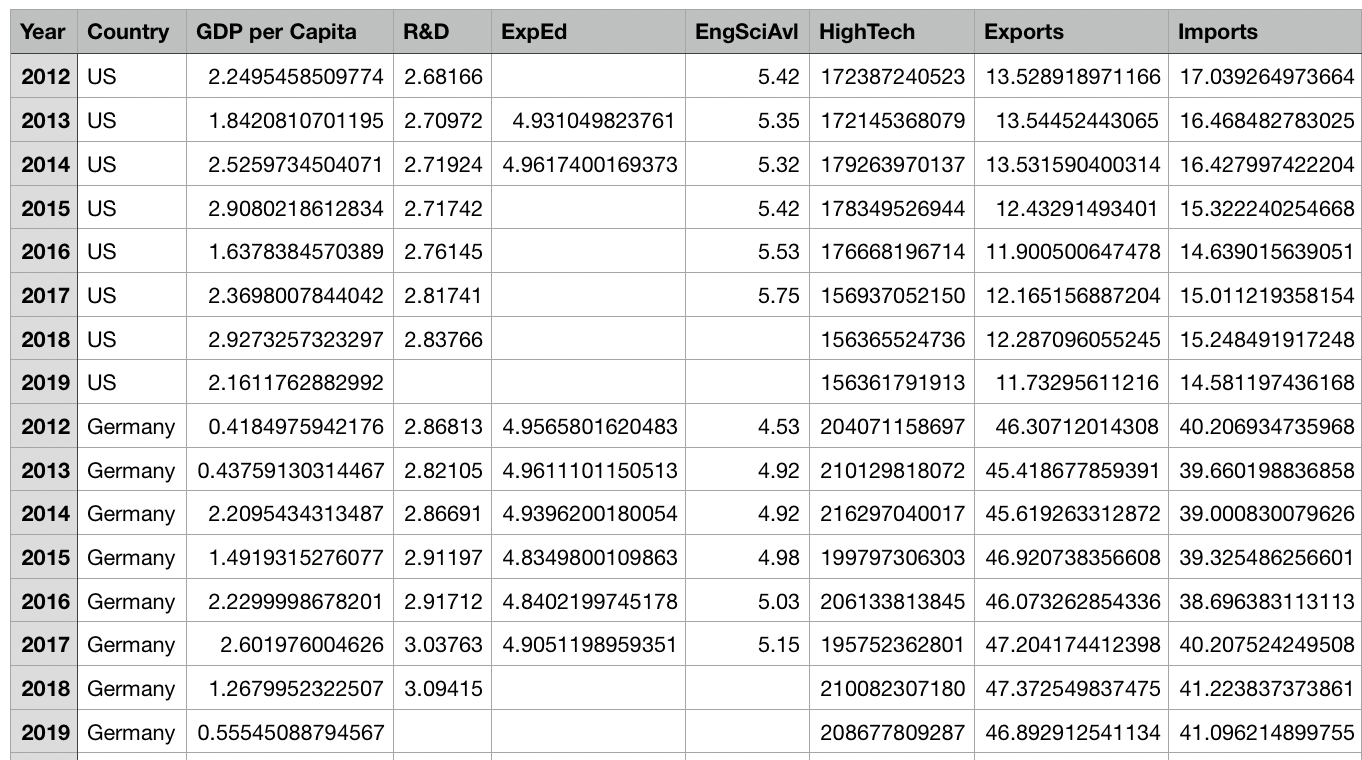
\includegraphics[scale=0.62]{dataset.png}
\caption{
        Dataset for Economies
    }
    \label{fig:basics AFM sketch}
\end{figure}

To read the data from the file ‘Economies.csv,’ we will be using the pandas data frame, which is a two-dimensional data structure with labeled rows and columns. Next, the $iloc()$ function within $pandas$, will help us retrieve a particular value or set of values belonging to a row and column using the index values assigned to it. The desired values of X (rows) and Y (columns) can be selected through this manner:

\begin{verbatim}
X = economies_pd.iloc[:, :-1]
Y = economies_pd.iloc[:, -1]
\end{verbatim}

The iloc() function and the sklearn model in $scikit-learn$ will be used to split the datqset into two parts: training set  and testing set (use X\_train, X\_test, y\_train, y\_test). 25\% of the data set will be used for training. The snippet of the code that will be used for this process is given below:

\begin{verbatim}
x_train, x_test, y_train, y_test = train_test_split(economies_pd.iloc[:, :-1],
economies_pd.iloc[:, -1],test_size = 0.25)
\end{verbatim}

\subsubsection{I. Training Set and Testing Set}
\hspace{20pt}Once the dataset has been split into training and testing data set, the lasso model will be imported from sklearn. The code snippet for this is as follows:

\begin{verbatim}
#import Lasso regression from sklearn library
from sklearn.linear_model import Lasso
  
#train the model
lasso = Lasso(alpha = 1)
lasso.fit(x_train, y_train)
y_pred1 = lasso.predict(x_test)

\end{verbatim}
As discussed earlier, the lasso model uses the L1 regularization by introducing a penalty called $\lambda$. To determine the accurate value of lambda, we will be using the k-fold cross-validation method (module: from sklearn.model\_selection import cross\_val\_score) and plot the cross-validation (CV) $R^2$ scores of the training and test data as a function of $\lambda$. The chosen lambda will have the highest $R^2$.
\vspace{50pt}

\begin{verbatim}
from sklearn.model_selection import cross_val_score
 
for ind, i in enumerate(lambdas):    
    reg = Lasso(alpha = i)
    reg.fit(X_train, y_train)
    results = cross_val_score(reg, X, y, cv=5, scoring="r2")
 
    train_r_squared[ind] = reg.score(X_train, y_train)    
    test_r_squared[ind] = reg.score(X_test, y_test)
 \end{verbatim}

\subsubsection{II. Plotting}
\hspace{20pt}A good visualization will help tell an easy-to-understand story. With our visualization tools, we aim to look at the trends and outliers that will further help derive insights crucial to the topic. There are multiple libraries in Python that will help us visualize our data. In this thesis, we will be using Matplotlib and Plotly. Matplotlib is the most popular data visualization library of Python and is a 2D plotting library. It has a versatile visualization library and is easy to use. The library enables us to create plots, bar charts, histograms, scatter plots, pie charts, etcetera. Plotly, on the other hand, is a web-based data visualization toolkit. It has a great Application Programming Interface (API) that makes it convenient to use. Some unique functionalities of Plotly include dendrograms and 3D charts along with scattered plots, contour plots, line charts, bar charts, etcetera. Using Plotly will help us visualize our results from the implementation of the lasso regression and the various values chosen for lambda to identify which value is the most accurate. Based on the results that we get, we can make inferences from our data regarding how SBTC and Globalization play a crucial role in affecting income inequality.



